\chapter{Développement}

\section{Modifications du framework}

Afin de pouvoir définir des tailles de sprite différentes et rectangulaires, nous avons créé notre propre classe OctolinkSpriteManager. Cela nous a également permi de créer des bounding box avec des tailles personnalisées et de bien les aligner par rapport aux sprites. Nous avons été obligé de dupliquer la classe IntersectTools du framework pour gérer les collisions correctement avec nos bounding box personnalisées.

\begin{figure}[ht!]
  \center
  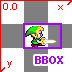
\includegraphics{resources/bbox.png}
  \caption{Link sprite bounding box}
  \label{fig:Link sprite bounding box}
\end{figure}


\section{Architecture du jeu}

\section{Fonctionnalites du jeu}

Ce jeu est un melange entre les jeux de types Tower Defence, et les jeux Zeldas. Le joueur a le controle de Link et a acces a tous les endroits du terrain de jeu, mis a part quelques obstacles comme les murs, ou comme l'eau.
Les Creeps, en revanche sont restraints au terrains de type "Path", comme dans certains Tower Defense, et ne peuvent en aucun cas quitter le chemin, et il est impossible de les y contraindre.\\
Il existe une condition de defaite, lorsque Zelda (destination finale des Creeps) n'a plus de points de vie, la partie est perdue.
La condition de victoire est d'eliminer tous les creeps que les Spawns prevoient d'envoyer a l'assaut de la princesse.
Link n'est lui meme pas invulnerable, il possede un certain nombre de points de vie lui aussi. S'il percute un mur (si il se fait ejecter dans un mur au contact d'un creep), il ne perdra pas de points de vie, mais il sera renvoye a son point d'apparition initiale.
Si ses points de vie atteindent zero, il sera egalement renvoye a son point d'origine, et son compteur de vie sera initialise a trois.\\
Link possede deux equipements: Son epee, et son bouclier.\\
Lorsque Link equipe son epee, il peut frapper les Creeps, ainsi les repoussant, et leur infligeant des degats.\\
Lorsque Link equipe son bouclier, il peut repousser les Creeps, de la meme maniere qu'avec l'epee, mais ce sans inflier de degats.\\


\section{Problèmes rencontrés}
